\documentclass[border=10pt]{standalone}
\usepackage{tikz}
\usepackage{amsmath}
\usetikzlibrary{arrows.meta, positioning, calc, fit, backgrounds, decorations.pathreplacing}

\begin{document}
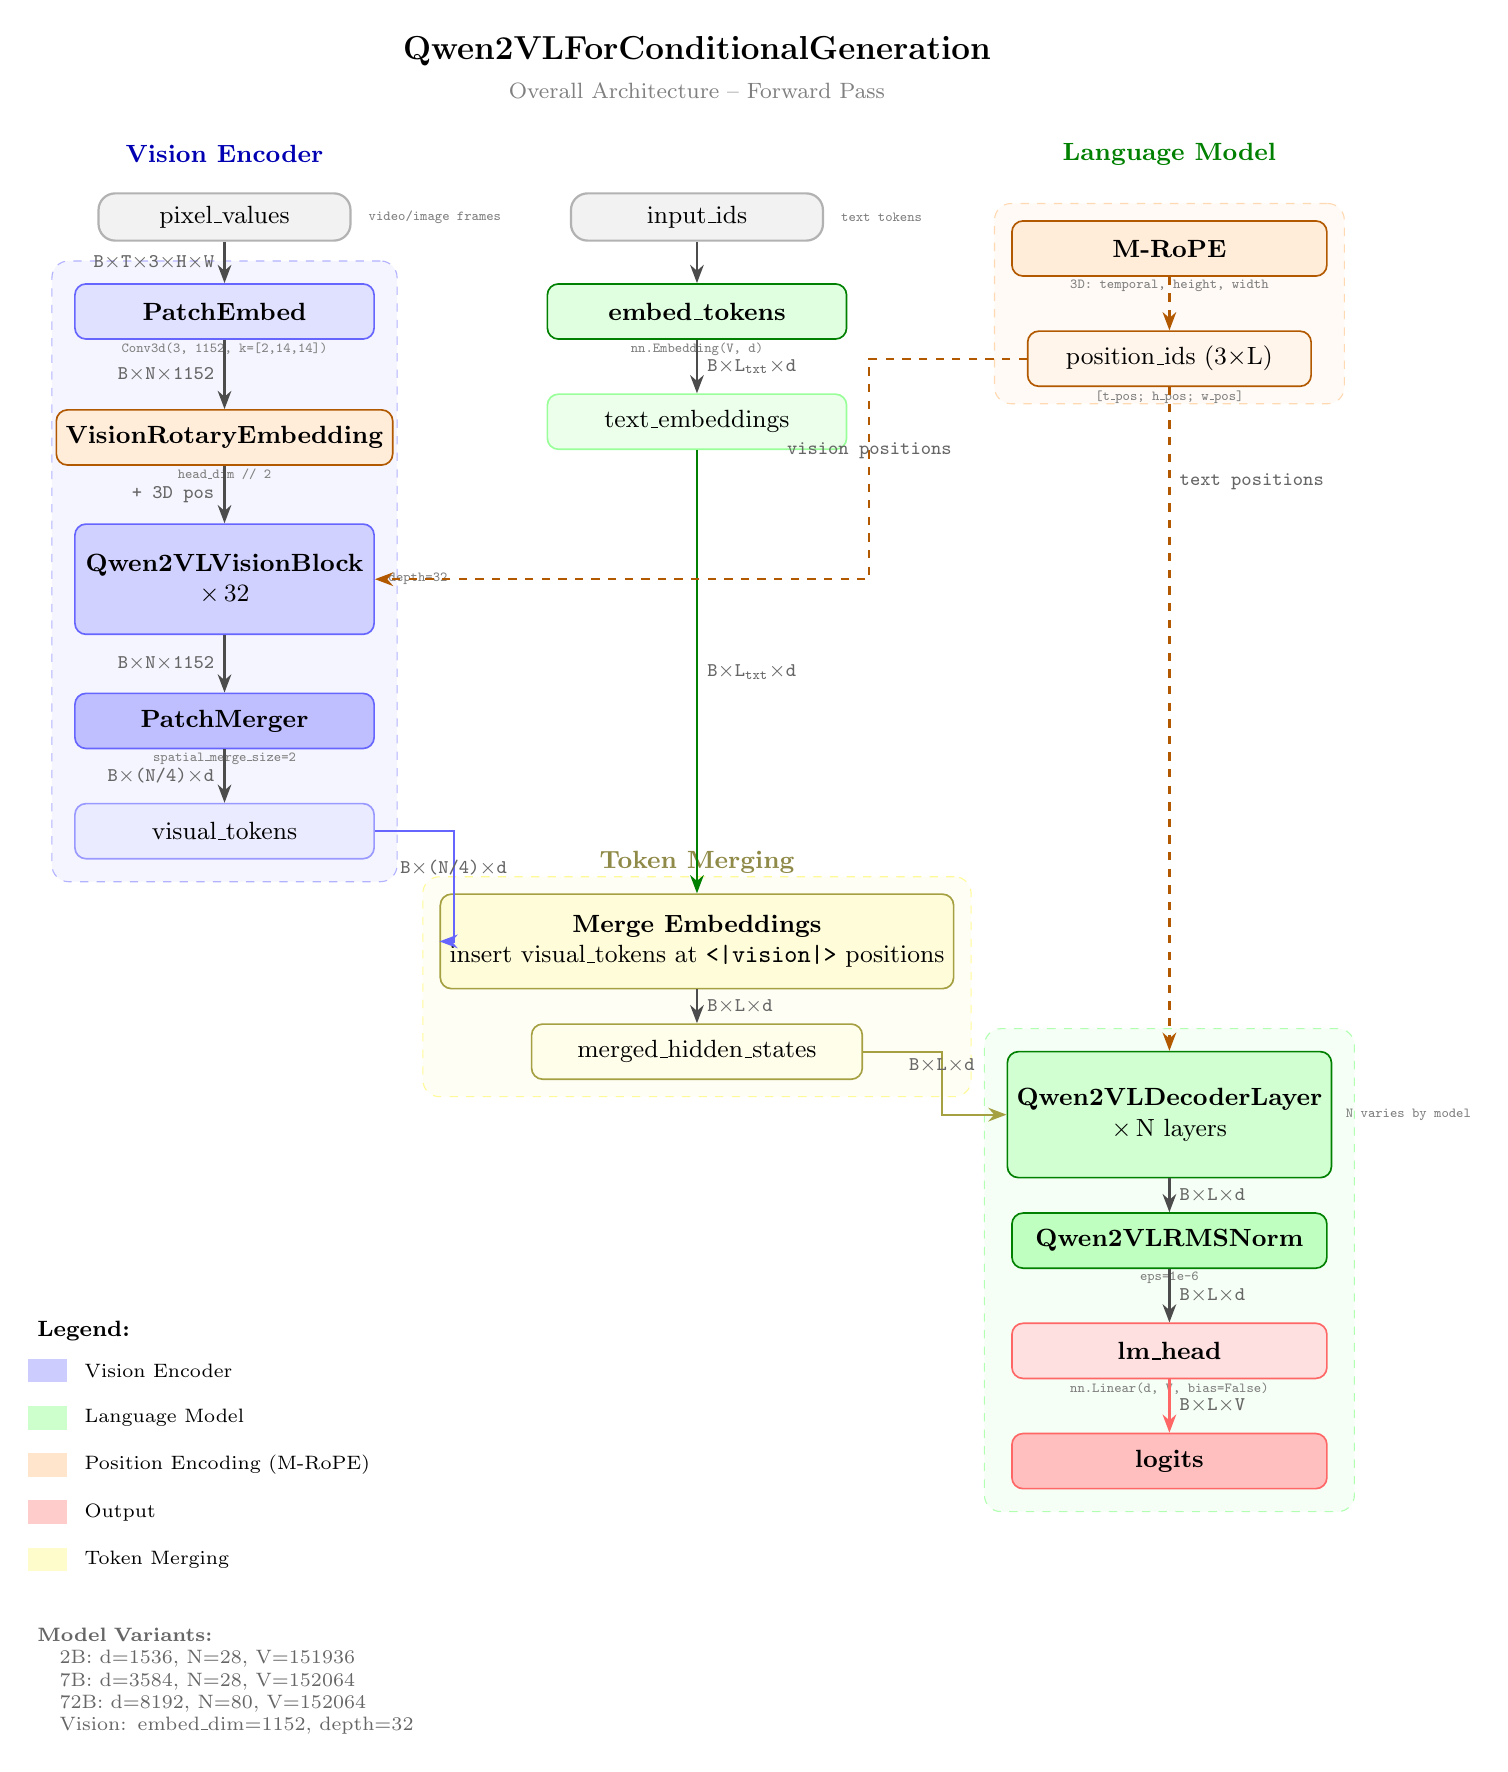
\begin{tikzpicture}[
    >=Stealth,
    node distance=0.7cm,
    % Style definitions
    vision/.style={draw, rounded corners=4pt, fill=blue!12, minimum width=3.8cm, minimum height=0.7cm, align=center, font=\small, line width=0.6pt, draw=blue!60},
    llm/.style={draw, rounded corners=4pt, fill=green!12, minimum width=3.8cm, minimum height=0.7cm, align=center, font=\small, line width=0.6pt, draw=green!50!black},
    posenc/.style={draw, rounded corners=4pt, fill=orange!15, minimum width=3.2cm, minimum height=0.7cm, align=center, font=\small, line width=0.6pt, draw=orange!70!black},
    output/.style={draw, rounded corners=4pt, fill=red!12, minimum width=3.8cm, minimum height=0.7cm, align=center, font=\small, line width=0.6pt, draw=red!60},
    merge/.style={draw, rounded corners=4pt, fill=yellow!15, minimum width=4.2cm, minimum height=0.7cm, align=center, font=\small, line width=0.6pt, draw=yellow!60!black},
    input/.style={draw, rounded corners=6pt, fill=gray!10, minimum width=3.2cm, minimum height=0.6cm, align=center, font=\small, line width=0.8pt, draw=gray!60},
    arrow/.style={->, thick, color=black!70},
    dimarrow/.style={->, thick, color=black!50},
    dimlabel/.style={font=\scriptsize\ttfamily, color=black!60},
    grouplabel/.style={font=\small\bfseries, color=black!80},
    annot/.style={font=\tiny\ttfamily, color=black!50},
    title/.style={font=\large\bfseries},
]

% ============================================================
% TITLE
% ============================================================
\node[title] (title) at (3.5, 17.5) {Qwen2VLForConditionalGeneration};
\node[font=\footnotesize, color=black!50] at (3.5, 17.0) {Overall Architecture -- Forward Pass};

% ============================================================
% LEFT: Vision Pipeline
% ============================================================
\node[grouplabel, blue!70!black] at (-2.5, 16.2) {Vision Encoder};

% Input
\node[input] (pixval) at (-2.5, 15.4) {pixel\_values};
\node[annot, right] at (pixval.east) {~video/image frames};

% PatchEmbed
\node[vision] (patemb) at (-2.5, 14.2) {\textbf{PatchEmbed}};
\node[annot, below=-0.08cm of patemb] (patemb_ann) {Conv3d(3, 1152, k=[2,14,14])};

% Vision RoPE
\node[posenc] (vrope) at (-2.5, 12.6) {\textbf{VisionRotaryEmbedding}};
\node[annot, below=-0.08cm of vrope] {head\_dim // 2};

% Vision Blocks
\node[vision, minimum height=1.4cm, fill=blue!18] (vblocks) at (-2.5, 10.8) {\textbf{Qwen2VLVisionBlock}\\$\times$\,32};
\node[annot, right=0.05cm of vblocks.east, anchor=west] {depth=32};

% PatchMerger
\node[vision, fill=blue!25] (merger) at (-2.5, 9.0) {\textbf{PatchMerger}};
\node[annot, below=-0.08cm of merger] {spatial\_merge\_size=2};

% Vision output
\node[vision, fill=blue!8, draw=blue!40] (vtokens) at (-2.5, 7.6) {visual\_tokens};

% Vision arrows
\draw[arrow] (pixval) -- (patemb) node[midway, left, dimlabel] {B$\times$T$\times$3$\times$H$\times$W};
\draw[arrow] (patemb) -- (vrope) node[midway, left, dimlabel] {B$\times$N$\times$1152};
\draw[arrow] (vrope) -- (vblocks) node[midway, left, dimlabel] {+ 3D pos};
\draw[arrow] (vblocks) -- (merger) node[midway, left, dimlabel] {B$\times$N$\times$1152};
\draw[arrow] (merger) -- (vtokens) node[midway, left, dimlabel] {B$\times$(N/4)$\times$d};

% ============================================================
% CENTER: Token Merging
% ============================================================
\node[grouplabel, yellow!50!black] at (3.5, 7.2) {Token Merging};

% Text input
\node[input] (textinp) at (3.5, 15.4) {input\_ids};
\node[annot, right] at (textinp.east) {~text tokens};

% Embed tokens
\node[llm] (embed) at (3.5, 14.2) {\textbf{embed\_tokens}};
\node[annot, below=-0.08cm of embed] {nn.Embedding(V, d)};

% Text embeddings
\node[llm, fill=green!8, draw=green!40] (textemb) at (3.5, 12.8) {text\_embeddings};

% Merge box
\node[merge, minimum height=1.2cm] (mergeop) at (3.5, 6.2) {\textbf{Merge Embeddings}\\insert visual\_tokens at \texttt{<|vision|>} positions};

% Arrows to merge
\draw[arrow] (textinp) -- (embed) node[midway, right, dimlabel] {};
\draw[arrow] (embed) -- (textemb) node[midway, right, dimlabel] {B$\times$L$_\text{txt}$$\times$d};
\draw[arrow, color=green!50!black] (textemb) -- (mergeop) node[midway, right, dimlabel] {B$\times$L$_\text{txt}$$\times$d};
\draw[arrow, color=blue!60] (vtokens.east) -- ++(1.0,0) |- (mergeop.west) node[near start, above, dimlabel] {B$\times$(N/4)$\times$d};

% Merged output
\node[merge, fill=yellow!8] (merged) at (3.5, 4.8) {merged\_hidden\_states};

\draw[arrow] (mergeop) -- (merged) node[midway, right, dimlabel] {B$\times$L$\times$d};

% ============================================================
% RIGHT: LLM Pipeline
% ============================================================
\node[grouplabel, green!50!black] at (9.5, 16.2) {Language Model};

% M-RoPE
\node[posenc, minimum width=4.0cm] (mrope) at (9.5, 15.0) {\textbf{M-RoPE}};
\node[annot, below=-0.08cm of mrope] (mrope_ann) {3D: temporal, height, width};

% Position IDs
\node[posenc, fill=orange!8, minimum width=3.6cm] (posids) at (9.5, 13.6) {position\_ids (3$\times$L)};
\node[annot, below=-0.08cm of posids] {[t\_pos; h\_pos; w\_pos]};

% Decoder layers
\node[llm, minimum height=1.6cm, fill=green!18, minimum width=4.0cm] (decoder) at (9.5, 4.0) {\textbf{Qwen2VLDecoderLayer}\\$\times$\,N layers};
\node[annot, right=0.05cm of decoder.east, anchor=west] {N varies by model};

% RMSNorm
\node[llm, fill=green!25, minimum width=4.0cm] (rmsnorm) at (9.5, 2.4) {\textbf{Qwen2VLRMSNorm}};
\node[annot, below=-0.08cm of rmsnorm] {eps=1e-6};

% lm_head
\node[output, minimum width=4.0cm] (lmhead) at (9.5, 1.0) {\textbf{lm\_head}};
\node[annot, below=-0.08cm of lmhead] {nn.Linear(d, V, bias=False)};

% Logits
\node[output, fill=red!25, minimum width=4.0cm] (logits) at (9.5, -0.4) {\textbf{logits}};

% LLM arrows
\draw[arrow, color=yellow!60!black] (merged.east) -- ++(1.0,0) |- (decoder.west) node[near start, above, dimlabel] {B$\times$L$\times$d};
\draw[arrow] (decoder) -- (rmsnorm) node[midway, right, dimlabel] {B$\times$L$\times$d};
\draw[arrow] (rmsnorm) -- (lmhead) node[midway, right, dimlabel] {B$\times$L$\times$d};
\draw[arrow, color=red!60] (lmhead) -- (logits) node[midway, right, dimlabel] {B$\times$L$\times$V};

% M-RoPE connections
\draw[arrow, dashed, color=orange!70!black] (mrope) -- (posids);
% M-RoPE to vision
\draw[arrow, dashed, color=orange!70!black] (posids.west) -- ++(-2.0,0) |- (vblocks.east)
    node[near start, above, dimlabel] {vision positions};
% M-RoPE to decoder
\draw[arrow, dashed, color=orange!70!black] (posids.south) -- ++(0,-1.2) -| ($(decoder.north)+(0.0,0)$)
    node[near start, right, dimlabel] {text positions};

% ============================================================
% Background groups
% ============================================================
\begin{scope}[on background layer]
    % Vision group
    \node[fit=(patemb)(vblocks)(merger)(vtokens)(patemb_ann), inner sep=8pt, fill=blue!4, draw=blue!30, rounded corners=6pt, dashed] (vgroup) {};
    % Merge group
    \node[fit=(mergeop)(merged), inner sep=6pt, fill=yellow!4, draw=yellow!40, rounded corners=6pt, dashed] {};
    % LLM group
    \node[fit=(decoder)(rmsnorm)(lmhead)(logits), inner sep=8pt, fill=green!4, draw=green!30, rounded corners=6pt, dashed] {};
    % Position group
    \node[fit=(mrope)(posids)(mrope_ann), inner sep=6pt, fill=orange!4, draw=orange!30, rounded corners=6pt, dashed] {};
\end{scope}

% ============================================================
% Legend
% ============================================================
\node[font=\footnotesize\bfseries, anchor=north west] at (-5.0, 1.5) {Legend:};
\fill[blue!20] (-5.0, 0.9) rectangle (-4.5, 0.6); \node[font=\scriptsize, anchor=west] at (-4.4, 0.75) {Vision Encoder};
\fill[green!20] (-5.0, 0.3) rectangle (-4.5, 0.0); \node[font=\scriptsize, anchor=west] at (-4.4, 0.15) {Language Model};
\fill[orange!20] (-5.0, -0.3) rectangle (-4.5, -0.6); \node[font=\scriptsize, anchor=west] at (-4.4, -0.45) {Position Encoding (M-RoPE)};
\fill[red!20] (-5.0, -0.9) rectangle (-4.5, -1.2); \node[font=\scriptsize, anchor=west] at (-4.4, -1.05) {Output};
\fill[yellow!20] (-5.0, -1.5) rectangle (-4.5, -1.8); \node[font=\scriptsize, anchor=west] at (-4.4, -1.65) {Token Merging};

% Parameter annotations
\node[font=\scriptsize, anchor=north west, text width=5cm, color=black!60] at (-5.0, -2.4) {
    \textbf{Model Variants:}\\
    \quad 2B: d=1536, N=28, V=151936\\
    \quad 7B: d=3584, N=28, V=152064\\
    \quad 72B: d=8192, N=80, V=152064\\
    \quad Vision: embed\_dim=1152, depth=32
};

\end{tikzpicture}
\end{document}
